\documentclass[10pt,a4paper]{article}
\usepackage[utf8]{inputenc}
\usepackage{geometry}
\geometry{left=20mm,top=20mm}

\usepackage{longtable}
\usepackage{tabularx} 
\usepackage{rotating}

\usepackage{pdflscape}
\usepackage{tabulary}                                                           
% Include the following packages 

\usepackage{array}
\usepackage{booktabs}  % for \toprule, \midrule, and \bottomrule macros 


\usepackage{float}
\usepackage{amsmath}
\usepackage{amsfonts}
\usepackage{amssymb}
\usepackage{color}
%\usepackage{multirow}

\usepackage{graphicx}
\usepackage{caption}
\usepackage{subcaption}




\usepackage{Sweave}
\begin{document}
\author{Giovana Gavidia, e-Health Unit, EURECAT}
\title{Predicting the next serum lactate based on vital sign time series and treatments}
\maketitle

\Sconcordance{concordance:lactate_APACHE_Tarragona.tex:lactate_APACHE_Tarragona.Rnw:%
1 31 1 1 0 13 1 1 12 1 23 1 1 1 8 1 86 16 1}


\tableofcontents

\listoffigures
% 
\listoftables




\section{Preprocessing}
\section {Initial Lactate vs. APACHE Analysis}

\begin{figure}[htp]
\begin{center}
  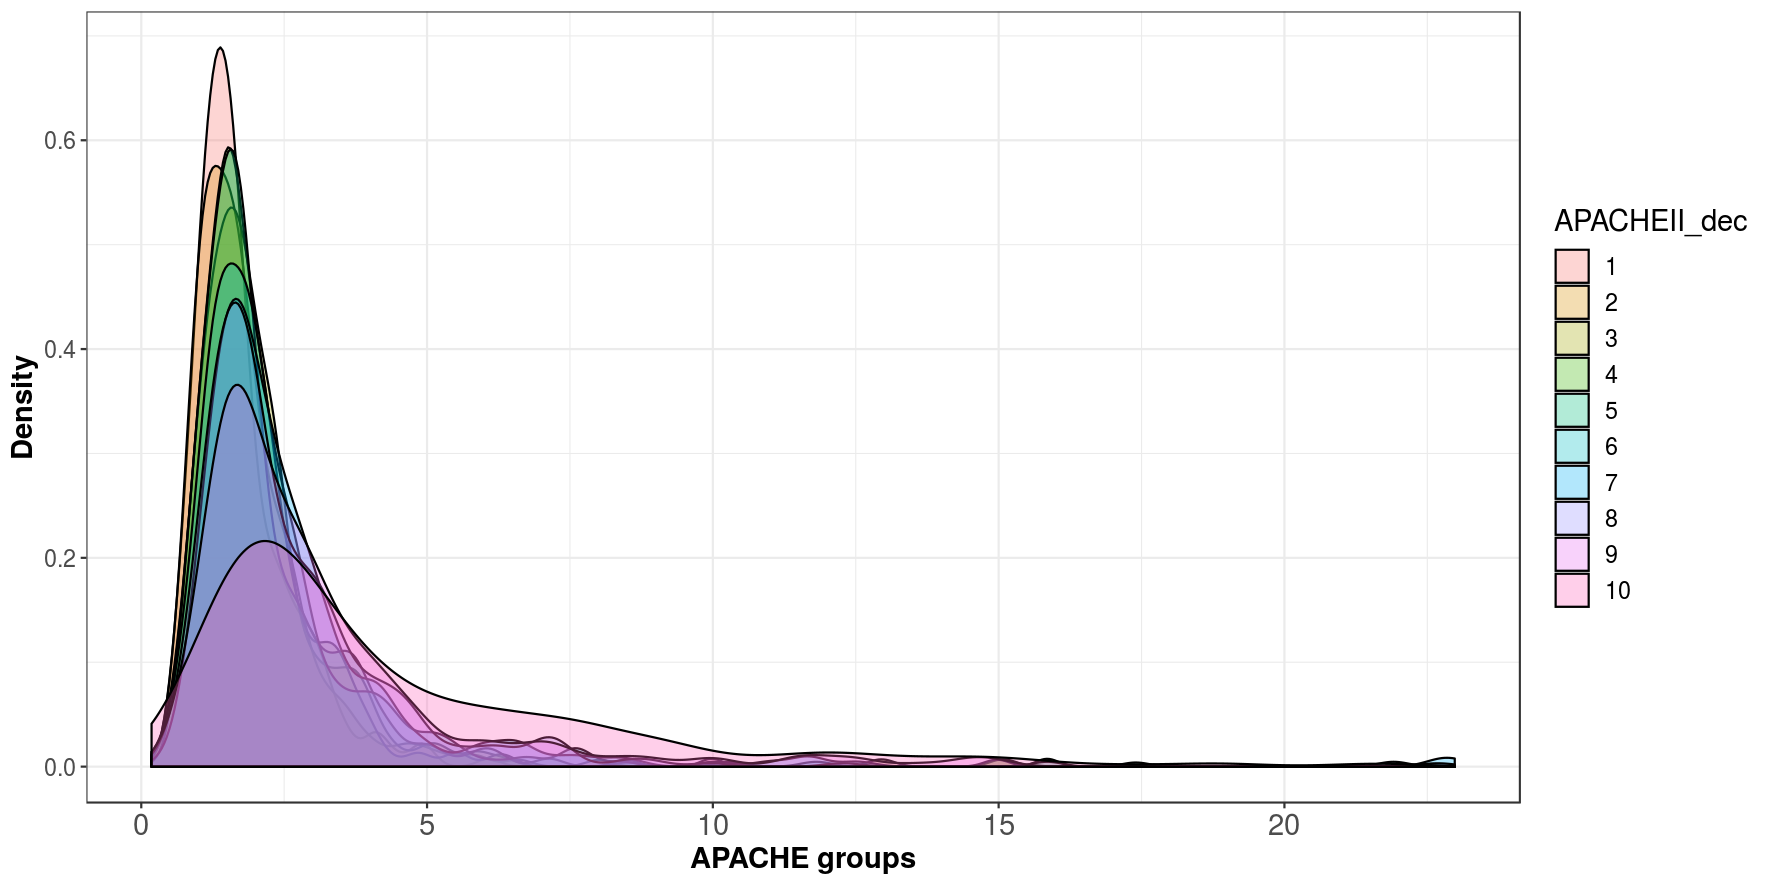
\includegraphics[width=14cm,height=23cm]{images/distribution_APACHEgroups.png}
\end{center}
\caption{Preprocessing steps. N represents the numbers of unique $icustay\_id$ and values inside brackets represent the numbers of unique $subject\_id$}
\label{fig:preprocessingPipeline}
\end{figure}

\begin{figure}[htp]
\begin{center}
  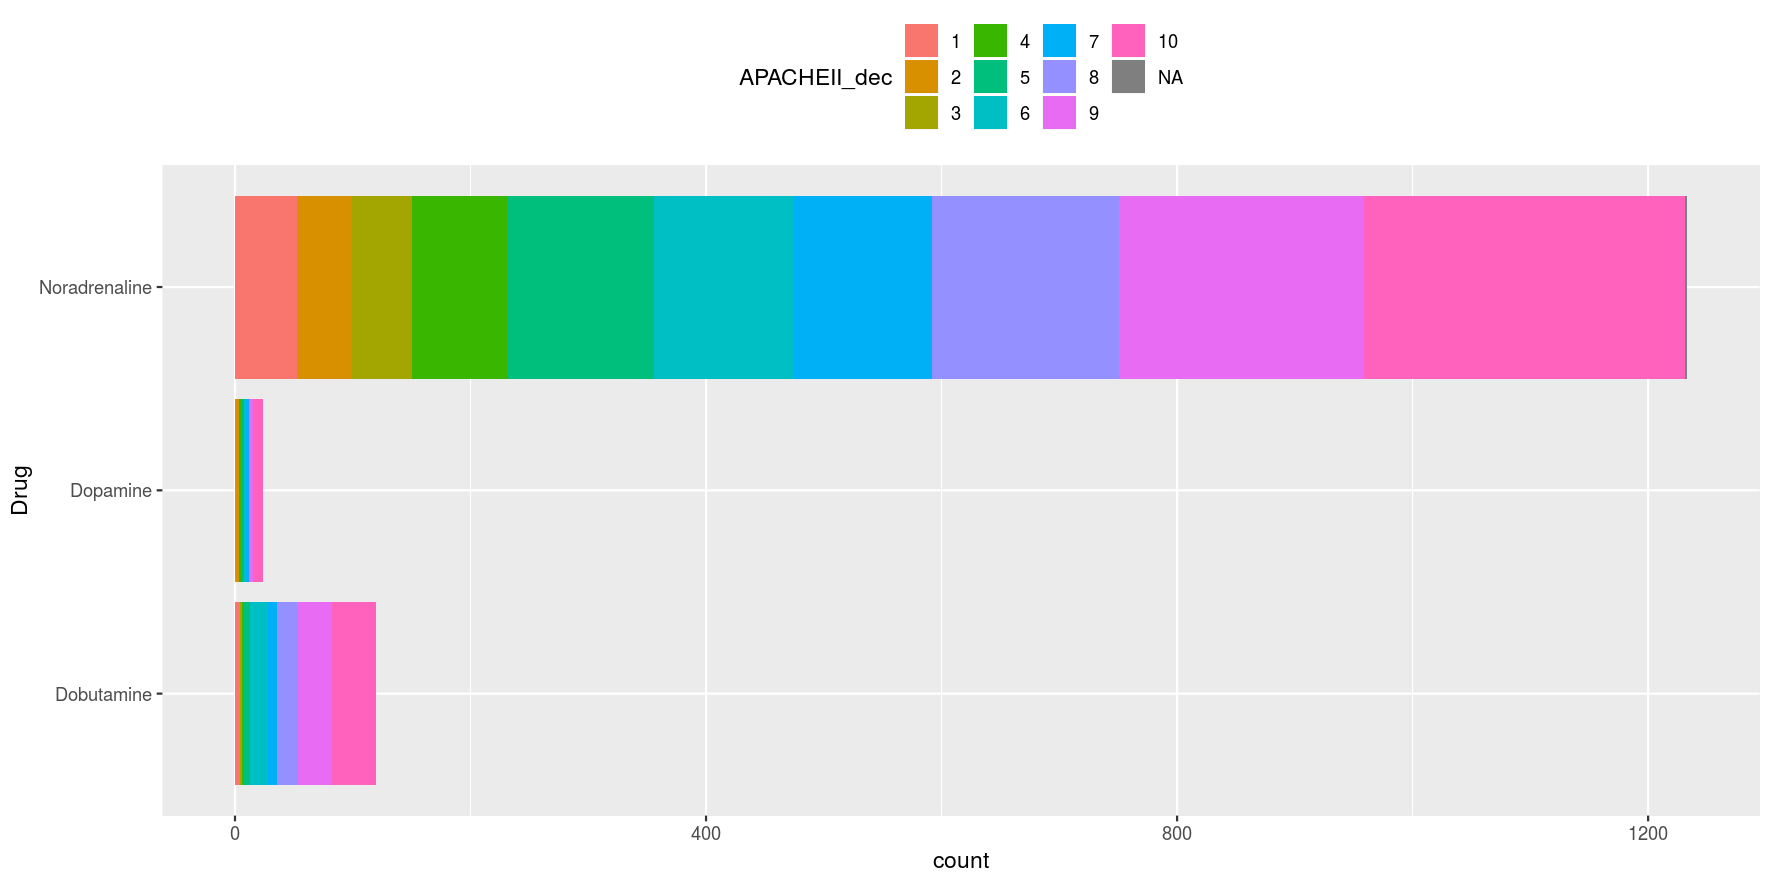
\includegraphics[width=14cm,height=23cm]{images/numberSamples_APACHEgroups.png}
\end{center}
\caption{Preprocessing steps. N represents the numbers of unique $icustay\_id$ and values inside brackets represent the numbers of unique $subject\_id$}
\label{fig:preprocessingPipeline}
\end{figure}
\end{document}
